\chapter{Lasery półprzewodnikowe}
\section{Teoria}
\subsection{Lasery półprzewodnikowe}
Lasery półprzewodnikowe są ważną oraz dynamicznie rozwijączą się gałęziom optoelektroniki. Znajduje one zastosowanie w telekomunikacji,
zapisie informacji. Wśród laserów połprzedwodnikowych możemy wyróżnić lasery o emisji krawędziowej oraz lasery typu VCSEL, które są przedmiotem
badań w mojej pracy. Obszarem czynnym w tego typów laserach są złącza p-n w którym obszar czynny jest pompowany przez przepływający prąd elektryczny
przez te złącza.
\subsection{Laser VCSEL}
Laser VCSEL (ang. \textit{Vertical Cavity Surface Emitting Laser}) są to lasery z emisją powierzchniową o pionowej wnęce rezonansowej.
Charakteryzują się możliwością emitowania promieniowania z dużej powierzchni, a rozkład poprzeczny promieniowania jest dowolny.
Inną ważną cechą, którą badam w swoje pracy jest mała wartość prądu progowego.
\subsection{Laser o emisji krawędziowej}
Lasery krawędziowe są to lasry z wnęka w  płaszczyźnie warstwy aktywnej. Charakteryzują się większą wartością prądu prowego
oraz większą sprawnością niż lasery VCSEL. Te cechy laserów są tematem moich badań.
\subsection{Prąd progowy}
Aby scharakteryzować lasery, można wykonać ich charakterystyki, które przedstawiają, jak zmienia się moc wyjściowa oraz napięcie lasera w funkcji zadanego prądu.
Przykładowe charakterystyki laserów pokazane są na rysunku \ref{teoria_rys_1}.
\begin{figure}
\center
  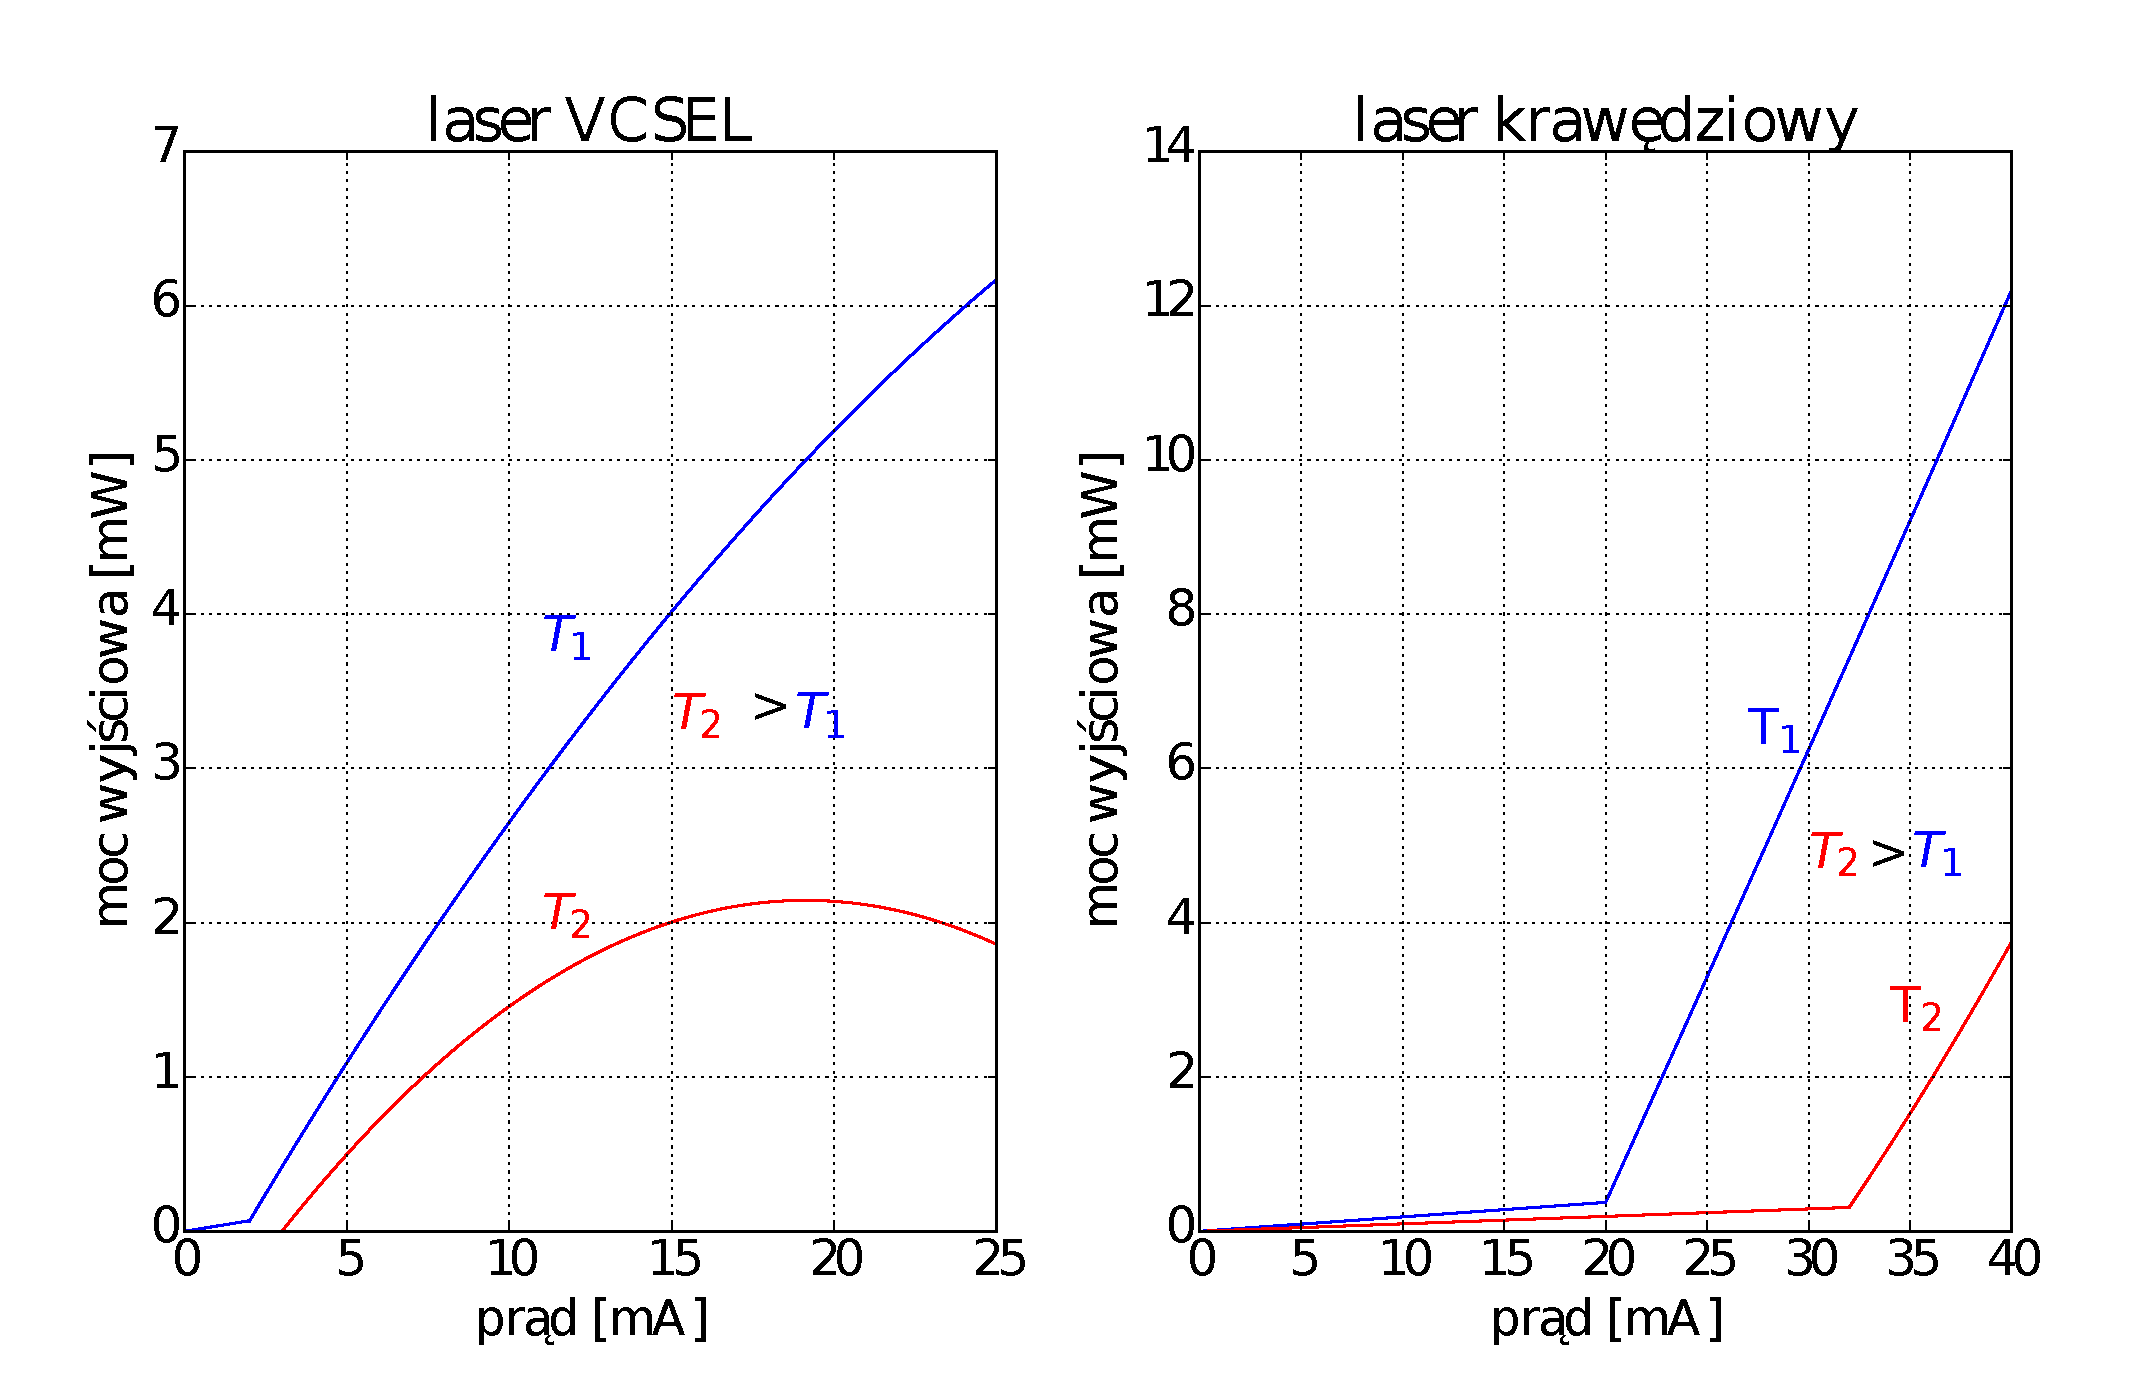
\includegraphics[scale=0.30]{wykres2.eps}
  \caption{Teoria.}
  \label{teoria_rys_1}
\end{figure}
Ważnym parametrem laserów półprzewodnikowych jest prąd progowy (z ang. \textit{threshold
current}) który określa wartość prądu, przy którym zaczyna zachodzić akcja laserowa, czyli
rośnie gwałtownie natężenie promieniowania i maleje szerokość linii emisyjnej. W celu wyznaczenia prądu progowego należy sporządzić wykres zależności mocy wyjściowej lasera od prądu zasilającego. Następnie dla prądu gdzie zaczyna się akcja laserowa dla odcinka liniowego należy metodą najmniejszych kwadratów przy użyciu wielomianu pierwszego stopnia znaleźć parametry krzywej. Dla wyznaczonej krzywej należy znaleźć miejsce zerowe, które będzie wyznaczonym prądem progowym.
\begin{equation}
P = a \cdot I + b
\end{equation}
\begin{equation}
I_{\mathrm{th}} = -\frac{b}{a}
\end{equation}
\begin{equation}
\Delta I_{\mathrm{th}} = \left\lvert \frac{\partial I_{th}}{\partial a} \right\rvert \cdot \Delta a + \left\lvert \frac{\partial I_{th}}{\partial b} \right\rvert \cdot \Delta b
\end{equation}
\begin{equation}
\Delta I_{\mathrm{th}} = \left\lvert -\frac{b}{a^2} \right\rvert \cdot \Delta a + \left\lvert -\frac{1}{a} \right\rvert \cdot \Delta b
\end{equation}
Dla laserów krawędziowych prąd progowy rośnie wraz z temperaturą, co może być scharakteryzowany za pomocą parametru
$T_{0}$ wyrażonego w kelwinach tzw. temperatury charakterystycznej ~\cite{opto_book}.
Dla laserów krawędziowych zależności prądu progowego $I_{th}$ od temperatury $T$ wyrażamy w postaci równania:
\begin{equation}
\label{eq:i_th}
I_{\mathrm{th}} = I_0 \exp \left( \frac{T}{T_0} \right)
\end{equation}
Wartości parametrów $I_0$ oraz $T_0$ możemy wyznaczyć na podstawie charakterystyk
emisyjnych lasera w różnych temperaturach $T$. \\
Przez zlogarytmowanie wartości prądu oraz podstawienie otrzymujemy:
\begin{equation}
\ln(I_{\mathrm{th}}) =    \frac{T}{T_0}  + \ln(I_0)
\end{equation}
Mając wartości prądu progowego w danej temperaturze  można do nich dopasować funkcje liniową w postaci:
\begin{equation}
y = a \cdot T + b
\end{equation}
Gdzie:
\begin{equation}
y = \ln(I_{\mathrm{th}})
\end{equation}
\begin{equation}
a = \frac{1}{T_0}
\end{equation}
\begin{equation}
b = \ln(I_0)
\end{equation}
Na tej podstawie możemy znaleźć poszukiwane parametry $I_0$ oraz $T_0$:
\begin{equation}
I_0 = \mathrm{e}^b
\end{equation}
\begin{equation}
T_0 = \frac{1}{a}
\end{equation}
Korzystając z różniczki zupełnej można obliczyć wartości błędów wyznaczonych wartości:
\begin{equation}
\Delta I_0 = \left\lvert \frac{\partial I_{0}}{\partial b} \right\rvert \cdot \Delta b = | \mathtt{e}^b | \cdot \Delta b
\end{equation}
\begin{equation}
\Delta T_0 = \left\lvert \frac{\partial T_{0}}{\partial a} \right\rvert \cdot \Delta a = \left\lvert -\frac{1}{a^2} \right\rvert \cdot \Delta a
\end{equation}
Dla laserów VCSEL nie można zastować powyszej zależności, ponieważ zależności prądu progowego od tempearury chrakteryzuje się pewnym
 minimalnym prądem progowym, gdzie w niższych i wyższych temperatuach wartość prądu progowego jest większa~\cite{publikacja_1}.
\subsection{Sprawność}
Innym ważnym parametrem, którym możemy scharakteryzować lasery półprzewodnikowe jest ich sprawność. Można wyróżnić następujące sprawności:
\begin{itemize}
\item Sprawność różniczkowa (ang. \textit{slope efficiency}) --- jest zdefiniowana jako nachylenie krzywej uzyskanej przez wykreślenie zależności
mocy wyjściowej z lasera versus energii dostarczonej do lasera w postaci natężenie prądu $I$ lub moc dostarczonej $P$.
Moc dostarczoną definujemy jako:
\begin{equation}
P = U \cdot I
\end{equation}
gdzie: $U$ --- napięcie na laserze.
\item Sprawność całkowita (ang. \textit{Wall-plug-efficiency}) --- jest zdefiniowana jako stosunek mocy wyjściowej do całkowitej mocy wejściowej lasera.
\end{itemize}
\subsection{Wpływ temperatury chłodnicy lasera na jego paramentry}
Wraz ze wzrostem temperatury wartość prądu progowego $I_{\mathrm{th}}$ rośnie, natomiast sprawność różniczkowa $\eta$ maleje. Jest to spowodowane przez:
\begin{itemize}
\item W wyższych temperaturach funkcja Fermiego-Diraca, która opisuje prawdopodobieństwo zajmowania stanów energetycznych staje się bardziej "rozmarzana". Przez co obrządzenie poziomów energetycznych jest bliższe powłoce przewodzenia dla elektronów oraz bliższe powłoce walencyjnej dla dziur. Dzięki temu możliwość wzmocnienia promieniowania lasera na długości fali emitowanej jest zredukowane.
\item Dodatkowo w podwójnym aktywnym regionie heterostruktury, rozkład energii elektronów i dziur w wyższych temperaturach jest przesunięty dalej od krawędzi pasma, przez co zwiększa się prawdopodobieństwo pobytu ładunków w aktywnym regionie, co powoduje obniżenie sprawności $\eta$
\item Wraz ze wzrostem temperatury rośnie współczynnik Auger, obniżając wydajność i czas życia ładunku podczas przejścia promienistego, co zwiększa wartość prądu progowego $I_{\mathrm{th}}$.
\end{itemize}
Sprawność różniczkowa zarówno dla laserów VCSEL i krawędziowych zwiększa się wraz z spadkiem temperatury chłodnicy lasera.
Jest to spodowane wyostrzaniem(ang. sharpening) się widma wzmocnienia na skutek zwężania się funkcji rozkładu Fermiego.
\subsection{Funkcja Fermiego}
Na wygłąd charakterystk laserów półprzewodnikowych duży wpływ ma funkcja rozkładu Fermiego-Diraca, który opisuje
własności półprzewodników jest ona zależna od temperatury. Opisuje prawdopodobieństwo obsadzenia przez elektron poziomu
energetynczego $E$ przy temperaturze $T$
\begin{equation}
f(E) = \frac{1}{e^{(E-E_F)/kT} + 1}
\end{equation}
gdzie: $E_f$ --- energia fermiego. \\
Wraz z wzrostem temperatury rośnie prawdopodobieństwo obszadzenia wyższego stanu energetynczego przez elektron. Ma to
wpływ na sprawność różniczkową laserów, wraz z wzrostem temperatury spraność ta maleje. Spowodowane jest to ostrzeniem
widma wzmocnienia, gdy rozkład fermiego się zweżą(narrowing)~\cite{publikacja_1}.
Poziom fermiego reprezentuje średnią pracę którą należy wykonać aby usunąć elektron z materiału.
\begin{figure}
\center
  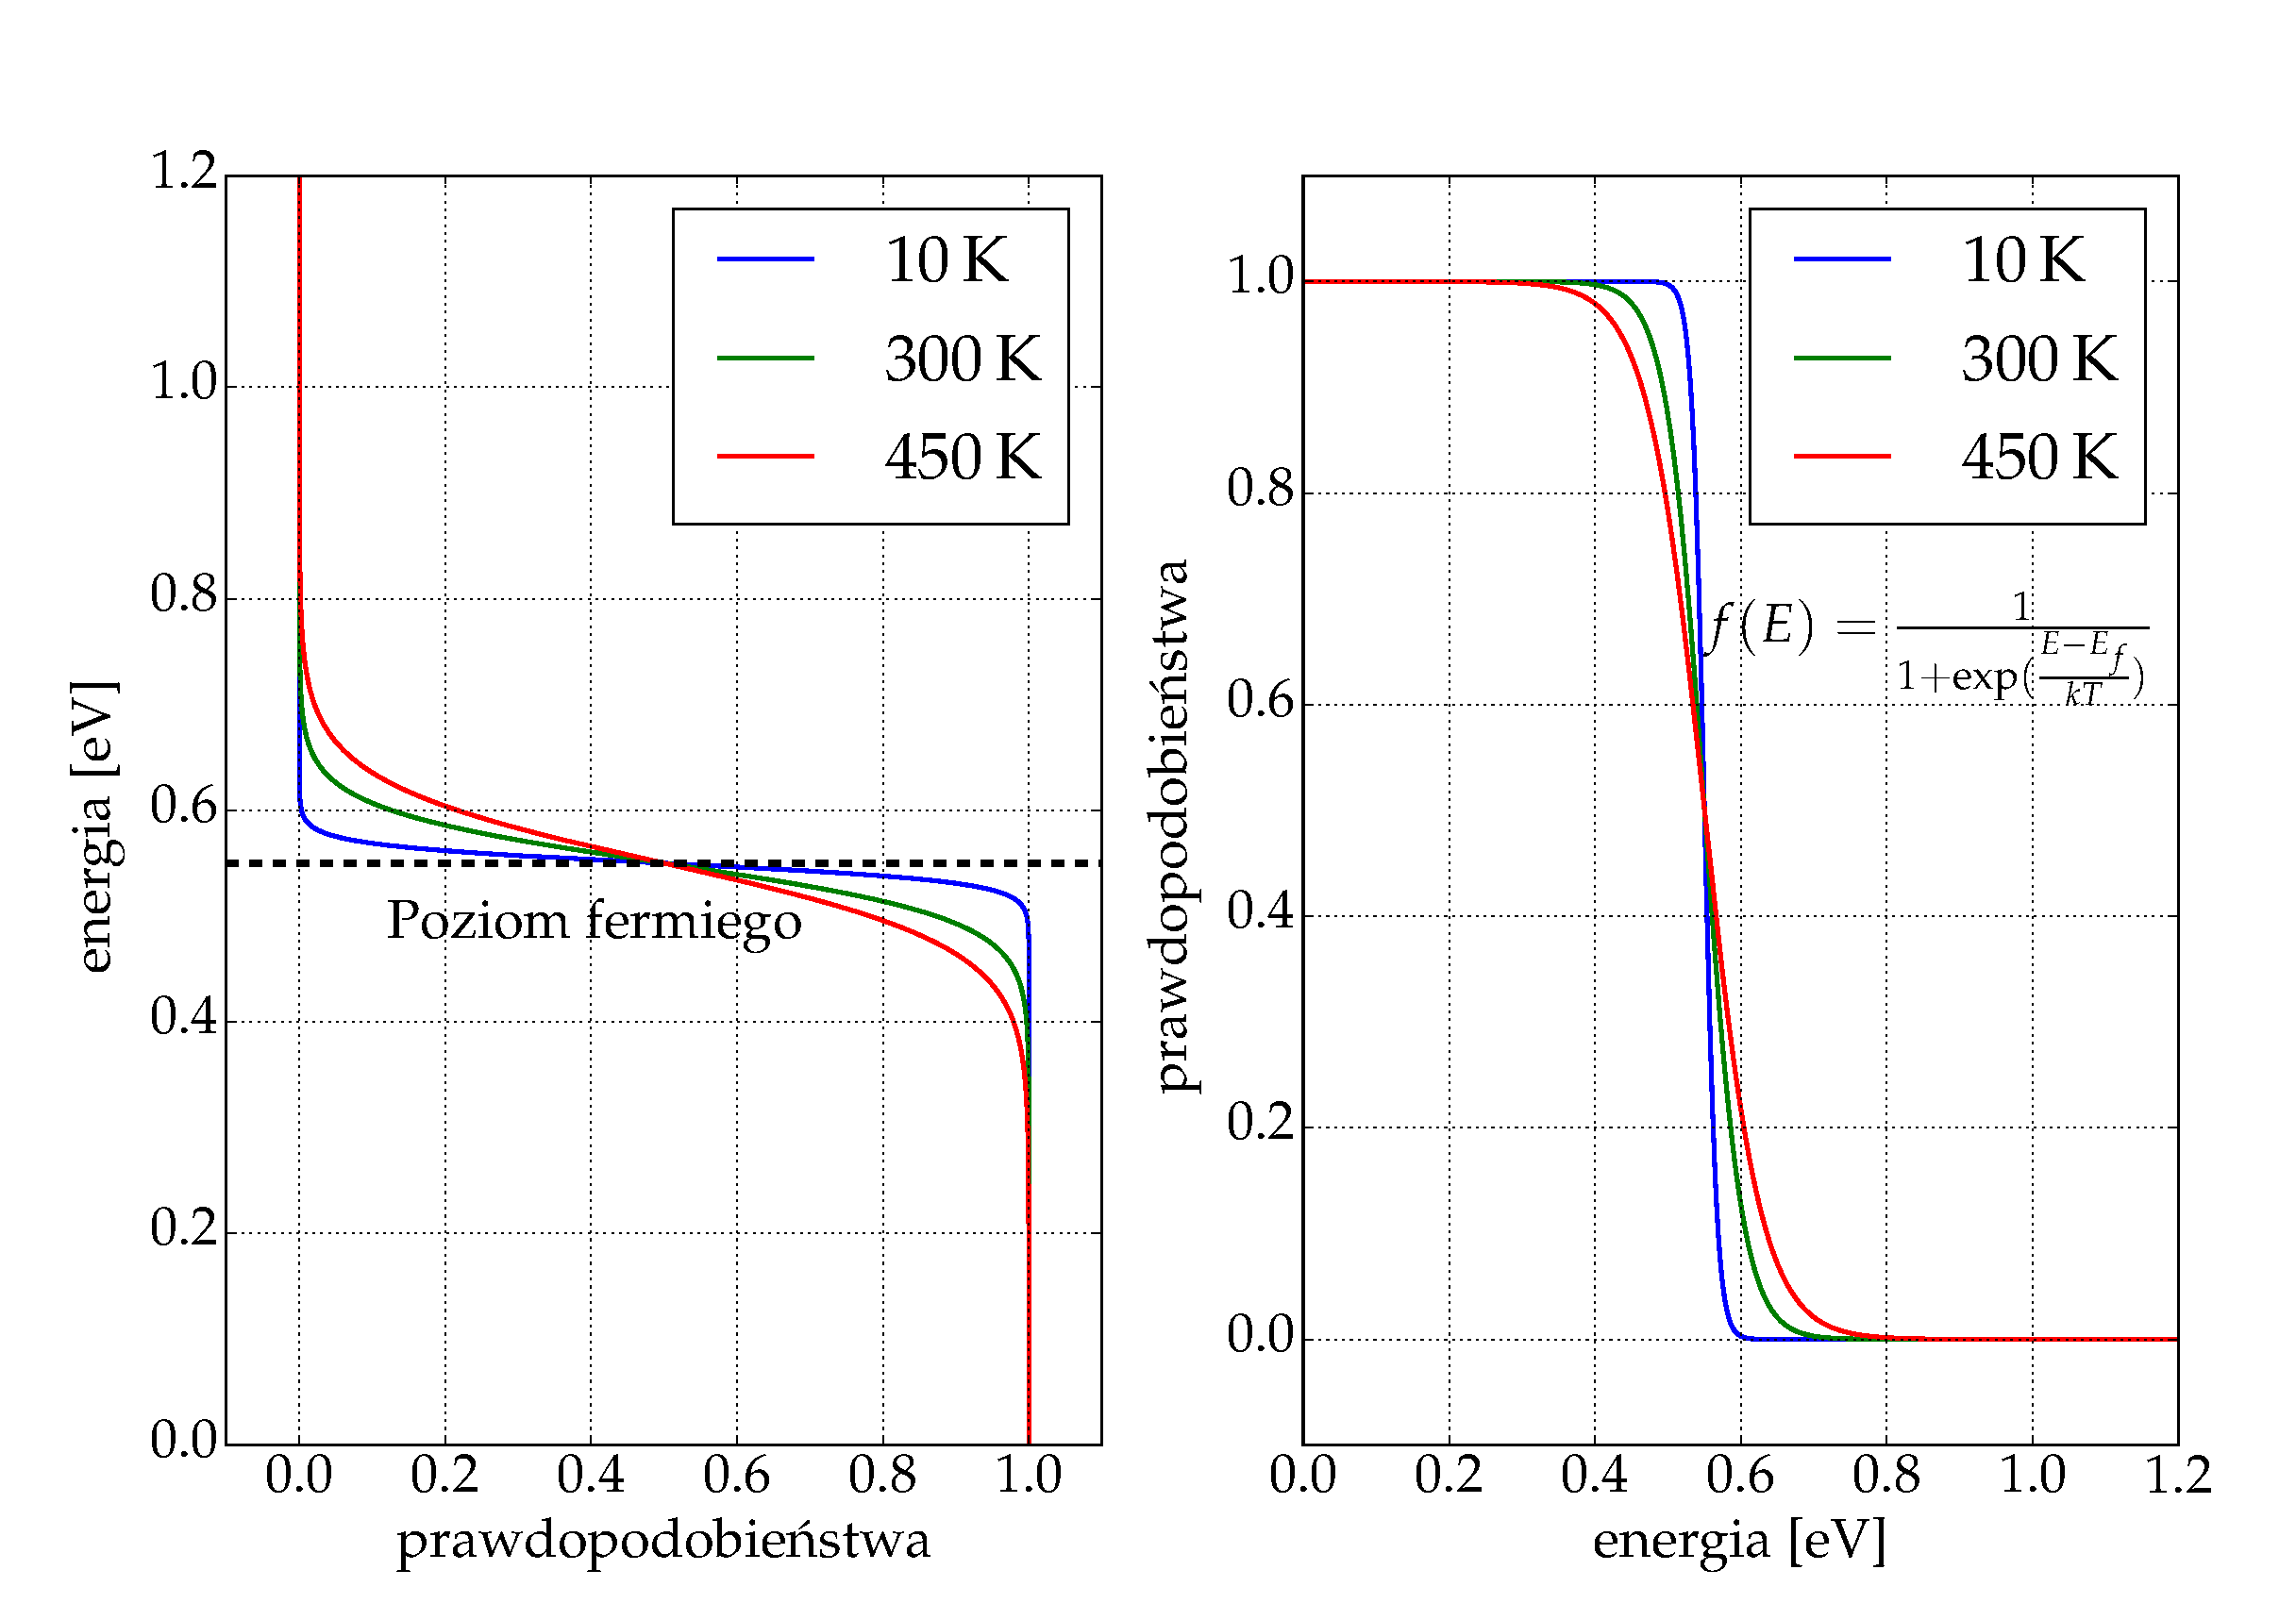
\includegraphics[scale=0.30]{fermi.eps}
  \caption{Rozkład fermiego dla różnych temperatur $T$.}
  \label{teoria_rys_1}
\end{figure}

\newpage